\section{Functions of Several Variables}

\subsection{Moving Through Dimensions}
We'll start with the most basic level. A simple line of real numbers. \\

\begin{center}
    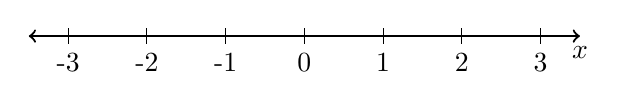
\begin{tikzpicture}
        \draw[thick, <->] (-3.5,0) -- (3.5,0) node[below] {$x$};

        \foreach \x in {-3,-2,-1,0,1,2,3}
            \draw (\x,0.1) -- (\x,-0.1) node[below] {\x};
    \end{tikzpicture}
\end{center}

We would represents the function as $\R$.

For two dimensions, we would would create two lines of real numbers and map them against each other.
\begin{center}
    \begin{tikzpicture}
        \draw[thick, <->] (-3.5,0) -- (3.5,0) node[below] {$x$};
    
        \draw[thick, <->] (0,-3.5) -- (0,3.5) node[left] {$y$};

        \foreach \x in {-3,-2,-1,1,2,3}
            \draw (\x,0.1) -- (\x,-0.1) node[below] {\x};
        
        \foreach \y in {-3,-2,-1,1,2,3}
            \draw (0.1,\y) -- (-0.1,\y) node[left] {\y};

    \end{tikzpicture}
\end{center}

For such a graph, we would represent the function as
\begin{align*}
    f : \R \rar \R
\end{align*}

Finally, for three dimensions we map a tuple of two to the real numbers.
\begin{center}
    \begin{tikzpicture}
        \draw[thick, <->] (-3.5,0,0) -- (3.5,0,0) node[below right] {$x$};
        \draw[thick, <->] (0,-3.5,0) -- (0,3.5,0) node[left] {$y$};
        \draw[thick, <->] (0,0,-3.5) -- (0,0,3.5) node[above] {$z$};

        \foreach \x in {-3,-2,-1,1,2,3}
            \draw (\x,0,0.1) -- (\x,0,-0.1) node[below] {\x};
        
        \foreach \y in {-3,-2,-1,1,2,3}
            \draw (0.1,\y,0) -- (-0.1,\y,0) node[left] {\y};

        \foreach \z in {-3,-2,-1,1,2,3}
            \draw (0,0.1,\z) -- (0,-0.1,\z) node[right] {\z};
    \end{tikzpicture}
\end{center}

Which we would represent with the function
\begin{align*}
    f : \R^2 \rar \R
\end{align*}

Or, for this course, it would be more helpful to think about these functions as,
\begin{align*}
    f(x,y) &= z
\end{align*}

We can formalize this definition as well.

\begin{definition}
    Suppose $f(x,y)$ is a \textbf{function of two variables}, then the set of all points $(x,y,z) \in \R^2$ such that $f(x,y) = z$ is the graph of
    $f(x,y)$ So, the points on teh graph are of the form $(x, y, f(x,y))$.
\end{definition}

Beyond the third dimension, graphical representations become difficult, but we can think about the relationships between input and outputs in terms of 
functions. For a function that maps $n$ variables to a real number, we would represent it as
\begin{align*}
    f : \R^n \rar \R.
\end{align*}

Or, more practically,
\begin{align*}
    f(x_1, ..., x_n) &= z.
\end{align*}

From now on, we'll focus primarily on three dimensions and generalizing formulas/tools to $n$ dimensions.

\subsection{Measuring Distance}
\begin{definition}
    Given two points $P_1(a_1, ..., a_n)$ and $P_2(b_1, ..., b_n)$, we can compute the \textbf{distance} with the following formula.
    \begin{align*}
        \sqrt{(b_1 - a_1)^2 + (b_2 - a_2)^2 + \cdots + (b_n - a_n)^2}
    \end{align*}
\end{definition}

\subsection{Generalizing Shapes}
We can start with shapes in lower dimensions and then express them in higher dimensions.

\begin{definition}
    \textbf{Translate} refers to the process of taking a function of fewer variables than dimensions and then extending it to more variables.
\end{definition}

\begin{definition}
    A \textbf{cylinder} refers to any function/shape that has been translated from its original dimensions to higher dimensions.
\end{definition}

For instance, if you were to take a point $x = 1$. You can translate it into $\R^2$ by representing it as the line $x = 1$.
Then, in three dimensions it would be a plane. In this case, the line and the plane are cylinders of the original point.

Similarly, you could start in the second dimension with a circle, then translate it into the third dimensions as a sphere. Here the sphere would
(somewhat counterintuitively) be the cylinder of the circle.

\subsection{Level Surfaces}
Sometimes it is difficult to graph a function by hand, so we rely on level surfaces.
\begin{definition}
    \textbf{Level surfaces} (sometimes known as \textbf{level curves}) are of the form
    \begin{align*}
        f(x,y) &= c \text{ for some constant $c \in \R$}
    \end{align*}

    \begin{example}
        Consider the function $f(x,y) = 100 - x^2 -y^2$.
        
        % \begin{center}
        %     \begin{tikzpicture}
        %         \begin{axis}[
        %             view={40}{40}, % Adjust the viewing angles
        %             colormap/viridis, % Color scheme
        %             axis lines=center,
        %             xlabel={$x$}, ylabel={$y$}, zlabel={$f(x,y)$},
        %             domain=-10:10,
        %             y domain=-10:10,
        %             samples=30, % Number of sample points
        %             samples y=30,
        %             enlargelimits=false,
        %             z buffer=sort
        %         ]
        %             \addplot3[surf] {100 - x^2 - y^2};
        %         \end{axis}
        %     \end{tikzpicture}
        % \end{center}

        For which the level curve would just be a bunch of circles. % upload graph maybe
    \end{example}

\end{definition}